\documentclass{article}
\usepackage{graphicx} % Required for inserting images
\usepackage[left=3cm, right=3cm, bottom=3cm, top=3cm]{geometry}	
\usepackage{setspace}
\onehalfspacing
\usepackage{float}
\usepackage{amsmath}

\title{Markowitz Portfolio Optimization with Inflation}
\author{Pablo Duce Cabeza, Djordje Nikolic, Sergey Mirzoev, Marc Tschudi}
\date{October 2023}

\begin{document}

\maketitle

\begin{figure}[h]
    \centering
    
\includegraphics[width=0.4\textwidth]{figure/uzh_logo_e_pos.eps}
    \label{fig:mesh0}
\end{figure}

\newpage
\tableofcontents
\newpage
\listoffigures
\listoftables
\newpage

\section{Introduction}


In an era marked by economic uncertainties and dynamic financial landscapes, the importance of constructing resilient investment portfolios cannot be underestimated. Investors face a constant challenge in preserving and enhancing the real value of their wealth, especially when confronted with the persistent threat of inflation. As inflation erodes purchasing power, traditional investment strategies may prove insufficient, necessitating a paradigm shift towards a more sophisticated approach.

This paper delves into the realm of portfolio optimization using the renowned Markowitz framework, with a specific focus on navigating the complexities of an inflationary environment. Rather than adhering to conventional wisdom, our methodology begins with a comprehensive analysis of various asset classes to discern their correlation with inflation. Recognizing that not all assets respond uniformly to inflationary pressures, we aim to identify and select those that not only weather the storm but offer a shield against the corrosive effects of rising prices.

The initial phase of our investigation involves an examination of different asset classes, ranging from equities and fixed income securities to commodities and real assets. By scrutinizing historical data and employing statistical techniques, we seek to unveil the intricate relationships between these asset classes and inflation. Our objective is to discern patterns and identify the investment instruments that exhibit a robust correlation with inflationary trends.

Building on this foundation, we move forward to the application of the Markowitz portfolio optimization model. Recognizing that optimal portfolios are not one-size-fits-all, we tailor our approach to incofixed-incomeunique characteristics of inflation-sensitive assets. Through a judicious combination of these assets, we aim to construct portfolios that not only maximize returns but, crucially, provide a hedge against the eroding effects of inflation.

As a result Markowitz'skowitz portfolio optimization under the specter of inflation, we show that a portfolio can be constructed which lies on the efficient frontier compared to an equally weighted portfolio. By strategically selecting assets that exhibit resilience in the face of inflation, the optimized portfolio outperforms an the CPI adjusted equally weighted portfolio substantially.

\newpage


\section{Asset Classes}

For an asset class to offer protection against inflation, the asset returns have to be positively correlated with the CPI (Consumer Price Index) when we assume that only long positions can be held; so, when the CPI increases, the asset returns should also increase. The approach we present will be based on filtering. Starting from a large pool of potential assets that could hedge against inflation, we want to understand what are the assets that are more prone to have a positive relationship with inflation. That means analyzing the yearly inflation rates, and see what are the subsequent returns of a given class. We therefore expect that besides high correlation with inflation, when inflation is very high, returns also should be very high (tail inflation corresponds with the tail of returns). We test the following asset classes and sectors for a hedge against inflation:

\begin{itemize}
    \item XHB: Median Sale Price of Houses Sold in the United States
    \item CPIAUCSL: Consumer Price Index for All Urban Consumers
    \item DCOILWTICO: Crude Oil Prices: West Texas Intermediate (WTI)
    \item GSPC: S\&P 500 Index
    \item GC=F: Gold Futures
    \item GS10: 10-Year Treasury Constant Maturity Rate
    \item GS30: 30-Year Treasury Constant Maturity Rate
    \item VNQ: REITs (Vanguard Real Estate ETF)
    \item DBC: Commodities (Invesco DB Commodity Index Tracking Fund)
    \item FXE: Foreign Currencies (Currency Shares Euro Trust)
    \item BTC-USD: Cryptocurrencies (Bitcoin)
    \item IGF: Infrastructure Funds (iShares Global Infrastructure ETF)
    \item XLE: Energy Stocks (Energy Select Sector SPDR Fund)
\end{itemize}

\subsubsection*{Visual inspection}

Visual inspection is a very quick way to determine if there's a relationship between the different asset classes. We look at the time series of the Log Returns of both the adjusted and non adjusted returns to see any potential relationships. Altough this is not very clear, it allows us to draw the first conclusions. In figure \ref{fig:mesh2} on page \pageref{fig:mesh2}, we can clearly see that bonds (GS10, GS30) are very very closely related and also follow CPI. We also can see a relationship between DBC (commodities) and XLE (energy).

\begin{figure}
    \centering
    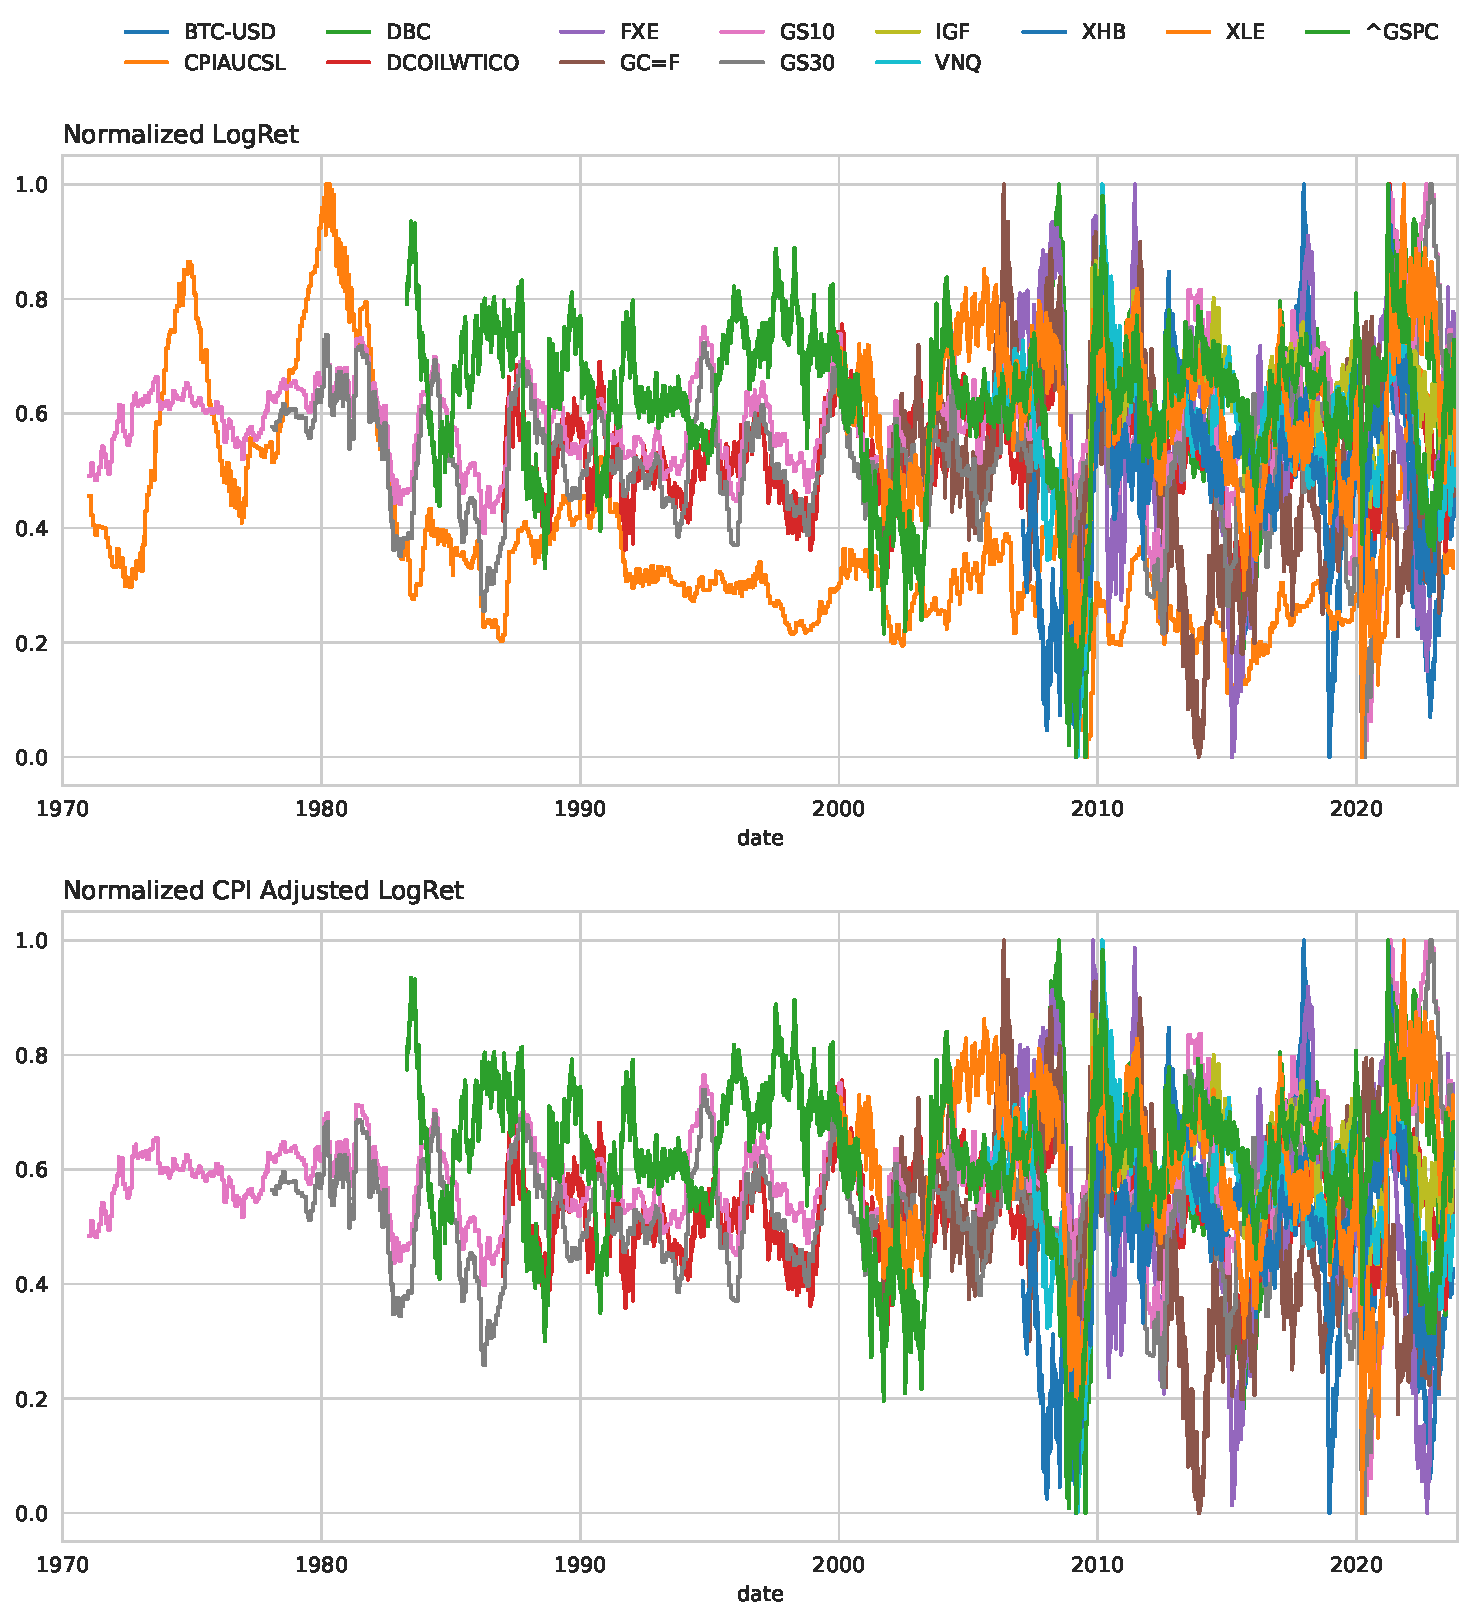
\includegraphics[width=1\textwidth]{figure/Normalized_Returns.pdf}
    \caption{Normalized Yearly Rolling Log-Returns of different Asset Classes.}
    \label{fig:mesh2}
\end{figure}



\subsubsection*{Correlation}

High correlation shows a linear relationship between the data. Using our data of yearly returns (rolling 1Y log returns) we can compute the pairwise correlation (correlation matrix). We are interested in the correlation between the CPI (CPIAUSCL) and a given asset class. The reason to compute the correlation in the returns and not in the prices, is that we can assume that returns are independent and identically distributed. Based on this result, we can observe that Energy ETF (XLE), Bonds (GS10, GS30), Oil (DCOILWTICO), Commodities (DBC)... are very postively correlated with inflation.

\begin{figure}[H]
    \centering
    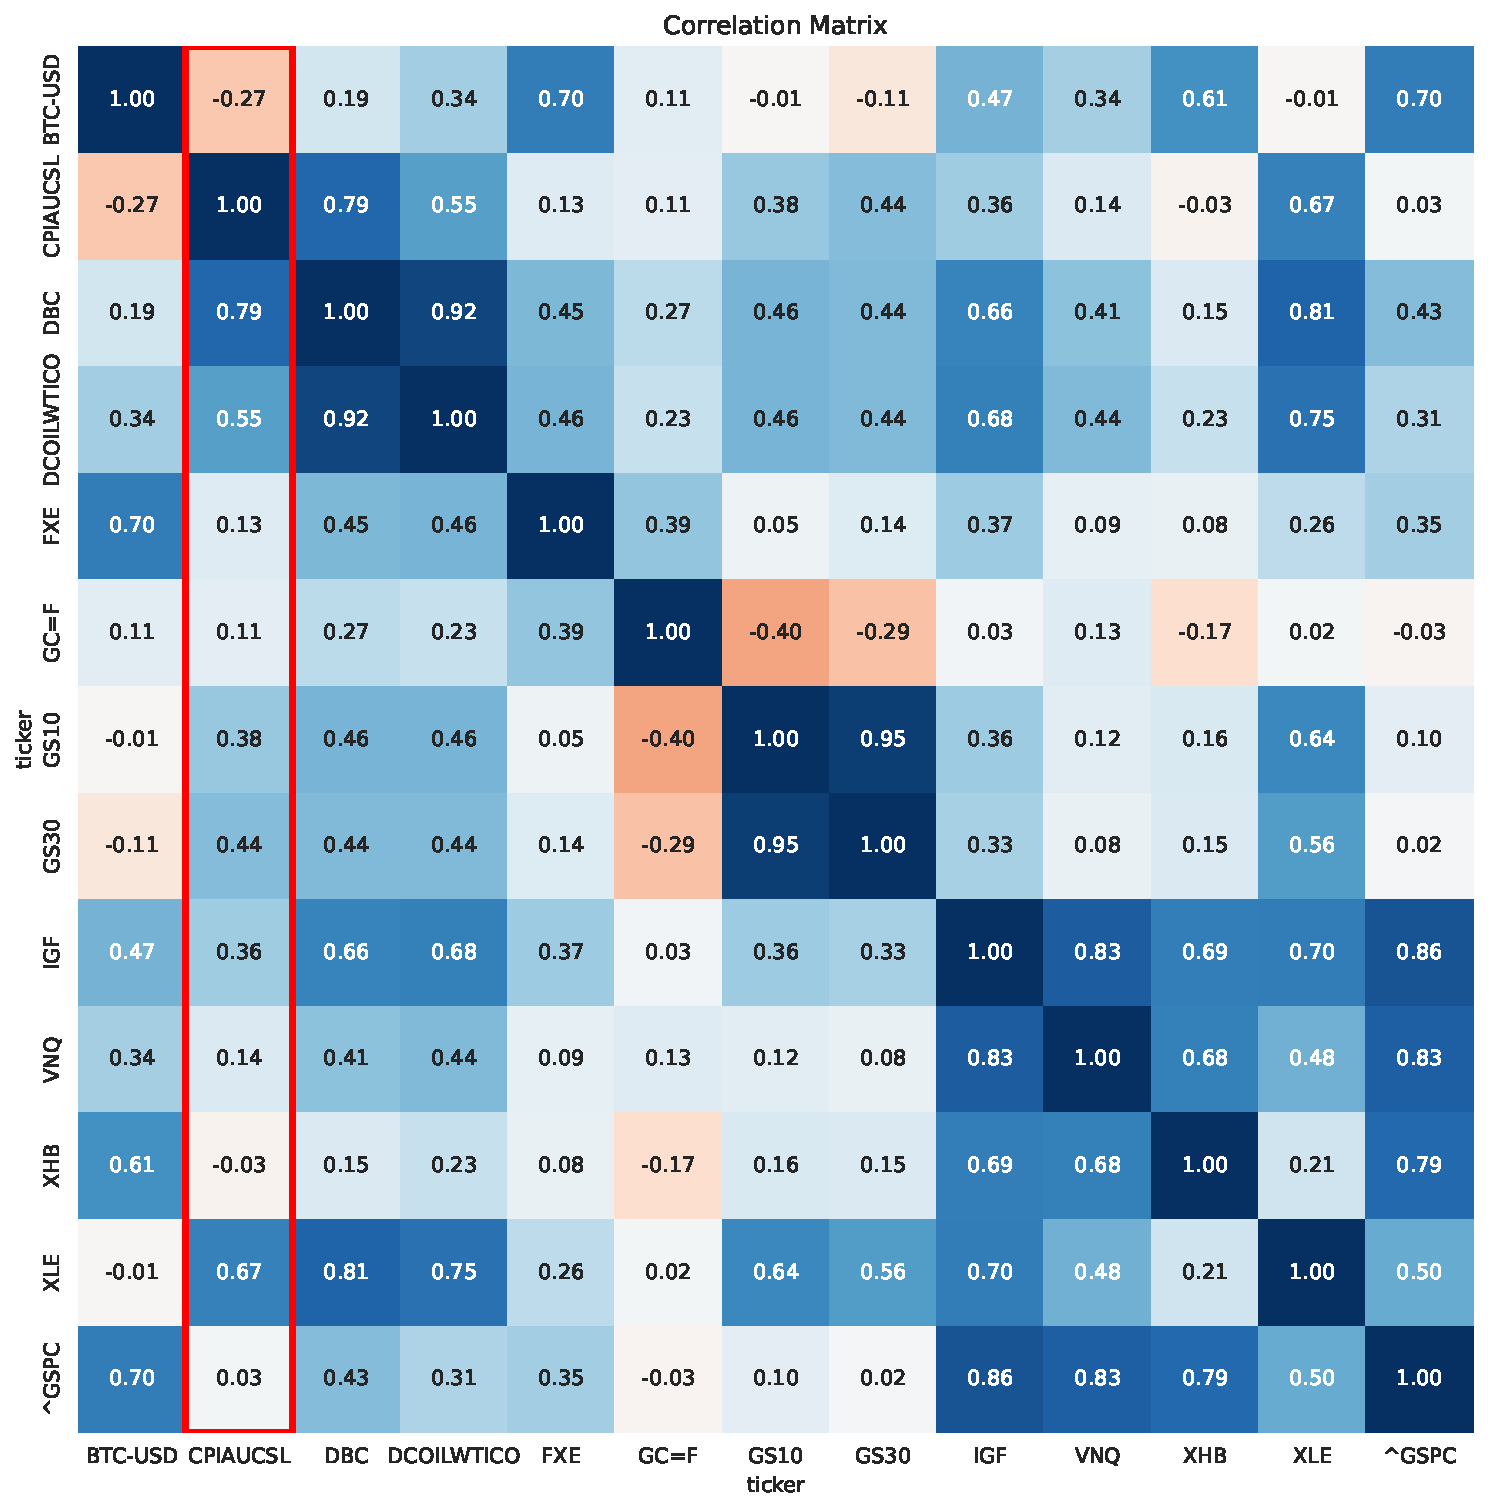
\includegraphics[width=0.8\textwidth]{figure/Correlation_Matrix.pdf}
    \caption{Correlation Matrix.}
    \label{fig:mesh1}
\end{figure}


\subsubsection*{Cointegration}

Based on the understanding of correlation in financial data, we can extend our analysis to explore the concept of cointegration. Cointegration is a statistical property of a collection of time series variables which indicates that a long-term equilibrium relationship exists between them. Unlike correlation that merely identifies the linear relationship in the level of data, cointegration delves deeper by detecting a link in their long-term trends, despite short-term deviations.

In our case, examining cointegration among assets like the Energy ETF (XLE), Bonds (GS10, GS30), Oil (DCOILWTICO), Commodities (DBC), and inflation metrics such as the CPI, would be insightful. This is particularly important because financial markets often exhibit trends and mean-reverting behavior over longer periods. While correlation informs us about the degree of linear relationship in the returns, cointegration helps us understand the extent to which these asset classes move together over time, bound by an equilibrium relationship.

By investigating cointegration, we can assess whether any discrepancies between these assets and inflation are temporary or indicative of a fundamental shift. This understanding is crucial for long-term investment strategies and risk management, as it helps in identifying pairs or groups of assets that are likely to move in sync over time. Such analysis is especially relevant in market conditions characterized by significant economic changes, where long-term relationships might be more stable and reliable compared to short-term correlations.

\begin{figure}[H]
    \centering
    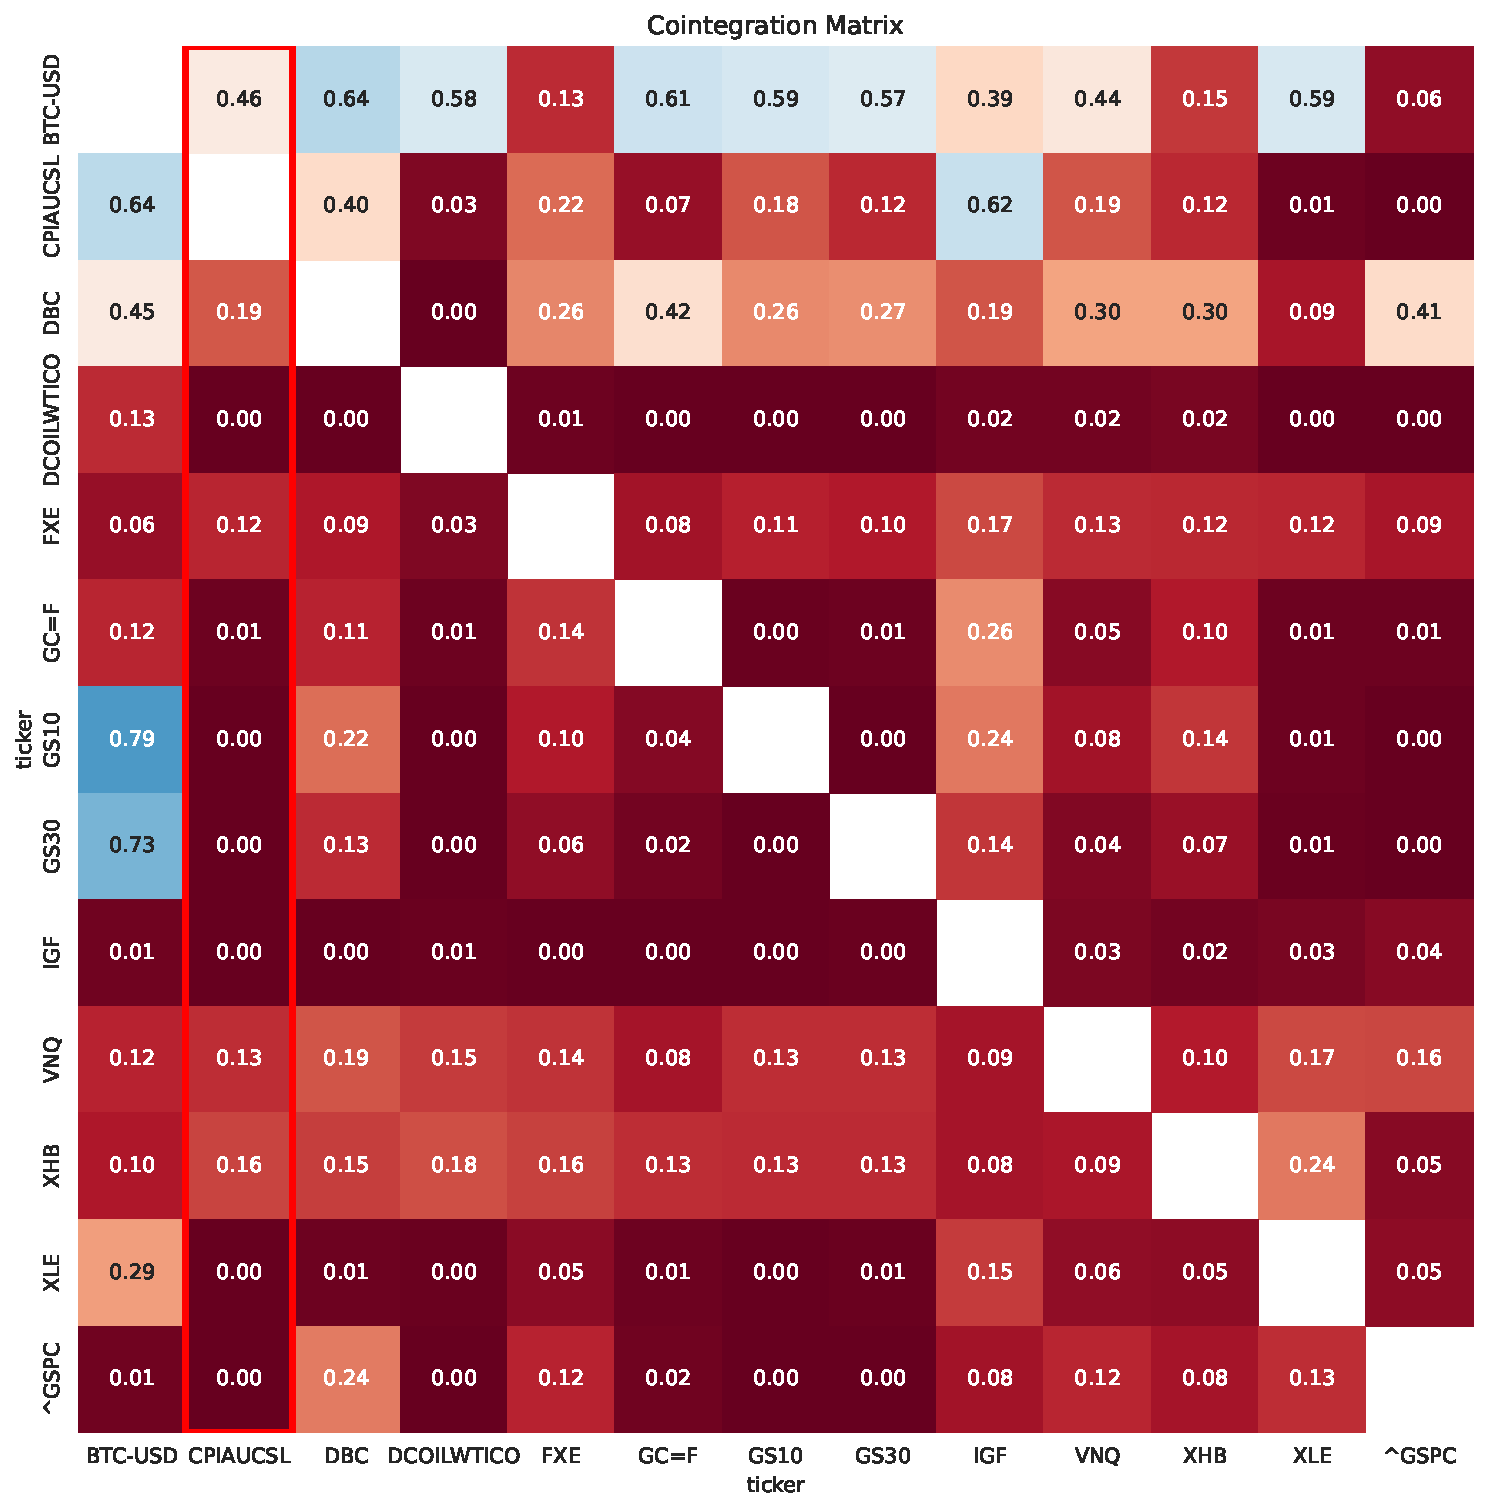
\includegraphics[width=0.8\textwidth]{paper/figure/Cointegration_Matrix.pdf}
    \caption{Cointegration Matrix.}
    \label{fig:mesh3}
\end{figure}

\section{Approach and Results}

In the following part we describe in more detail our approach as well as the results. 

\subsection{The Concept of Portfolio Optimization}

\subsubsection*{Efficient Frontier}

The heart of Markowitz's theory is the "Efficient Frontier," a graphical representation showing the optimal set of portfolios providing the maximum possible expected return for a given level of risk. Portfolios that lie below the efficient frontier are sub-optimal because they do not provide enough return for the level of risk they carry.

\subsubsection*{Risk and Return}

In Markowitz's framework, risk is quantified as the standard deviation of portfolio returns, a measure of variability in returns. Return is the expected return of the portfolio, a weighted sum of the expected returns of the individual assets.

\subsection{Mathematical Formulation}

\subsubsection*{Expected Portfolio Return}

The expected return of a portfolio is the weighted sum of the returns of the individual asset classes:

\begin{equation}
R_p = \sum_{i=1}^{n} w_i \times R_i
\end{equation}

where \( R_p \) is the expected portfolio return, \( n \) is the number of assets in the portfolio, \( w_i \) is the weight of the asset \textit{i}, and \( R_i \) is the expected return of the asset \textit{i}.


\end{document}
